%\documentclass[11pt,aspectratio=169]{beamer}
\documentclass[11pt]{beamer}
\usetheme{Darmstadt}
%\usecolortheme{dolphin}

%\setbeameroption{show notes}
%\setbeameroption{show only notes}
%\usepackage{pgfpages}
%\pgfpagesuselayout{4 on 1}[a4paper,border shrink=5mm]

\usepackage[utf8]{inputenc}
\usepackage[english]{babel}
\usepackage{amsmath}
\usepackage{amsfonts}
\usepackage{amssymb}
\usepackage{graphicx}
\usepackage{subcaption}
\usepackage{algorithmic}
\captionsetup{compatibility=false}

\author{Andrew Rosen}
\title[DHT Distributed Computing]{Proposal \\ Towards a Framework for DHT Distributed Computing}

\logo{
\includegraphics[height=1cm]{figs/logo}}
\institute{Georgia State University}
\date{July 15th, 2015}
%\subject{}
%\setbeamercovered{transparent}
%\setbeamertemplate{navigation symbols}{}



\AtBeginSection[]
{
  \begin{frame}
    \frametitle{Table of Contents}
    \tableofcontents[currentsection]
  \end{frame}
}

\begin{document}
	
	
	
\maketitle


\section{Introduction}


\subsection{Objective}
\begin{frame}{Objective}
Our objective is to create a generalized framework for distributed computing using Distributed Hash Tables.

\pause
\begin{center}
	Or
\end{center}

\pause
We want to build a completely decentralized distributed computing framework.
\end{frame}

\note[itemize]{
	\item We want to build a completely decentralized distributed computing framework based on distributed hash tables, or DHTs.
	\item Doing this will require a generic framework for creating 	distributed hash tables and distributed applications
}

\subsection{Distributed Computing and Challenges}

\begin{frame}{What do I Mean by Distributed Computing?}
	A system where we can take a task and break it down into multiple parts, where each part is worked upon individually.
\end{frame}

\note{A distributed computing framework is a system where we can take a job, break in up into smaller pieces, and send these pieces out to be worked upon by computing agents.}

\begin{frame}{Challenges of Distributed Computing}
	Distributed Computing platforms experience these challenges:
	\begin{description}
		\item<1->[Scalability] As the network grows, more resources are spent on maintaining and organizing the network. 
		\note<1>{Remember, computers aren't telepathic. There's always an overhead cost.  It will grow.   The challenge of scalability is designing a protocol  in which this cost grows at an extremely slow rate. 
			For example, a single node keeping track of all members of the system might be a tenable situation up to a certain point, but eventually, the cost becomes too high for a single node.}
		\item<2->[Fault-Tolerance] As more machines join the network, there is an increased risk of failure. \note<2>{Failure Hardware failure is a thing that can happen. Individually the chances are low, but this becomes high when we're talking about millions of machines.  Also, what happens in a P2P environment.}  
		\item<3->[Load-Balancing] Tasks need to be evenly distributed among all the workers. \note<3>{If we are splitting the task into multiple parts, we need some mechanism to ensure that each worker gets an even (or close enough) amount of work.}
	\end{description}
	
\end{frame}


\subsection{What Are Distributed Hash Tables?}

\begin{frame}{Distributed Key/Value Stores}
	\textbf{Distributed Hash Tables }are mechanisms for storing values associated with certain keys.
	\begin{itemize}
		\item Values, such as filenames, data, or IP/port combinations are associated with keys.
		\item These keys are generated by taking the hash of the value.
		\item We can get the value for a certain key by asking any node in the network.
	\end{itemize}
\end{frame}


\begin{frame}{Current Applications}
	Applications that use or incorporate DHTs:
	\begin{itemize}
		\item P2P File Sharing applications, such as BitTorrent.
		\item Distributed File Storage.
		\item Distributed Machine Learning.
		\item Name resolution in a large distributed database.
	\end{itemize}
\end{frame}


\begin{frame}{How Does It Work?}
	We'll explain in greater detail later, but briefly:
	\begin{itemize}
		\item DHTs organize a set of nodes, each identified by an \textbf{ID}. \note{We use ID for nodes and keys for data so we always know our context.}
		\item Nodes are responsible for the keys that are closest to their IDs.
		\item Nodes maintain a list of other peers in the network.
		\begin{itemize}
			\item Typically a size $ \log(n)$ subset of all nodes in the network.
		\end{itemize}
		\item Each node uses a very simple routing algorithm to find a node responsible for any given key.  %Explain what that is
	\end{itemize}
\end{frame}



%\begin{frame}{Strengths of DHTs }
%	DHTs are designed for large P2P applications, which means they need to be (and are):
%	\begin{itemize}
%		\item[Scalable] 
%		\begin{itemize}
%			\item Each node knows a \emph{small} subset of the entire network.
%			\item Join/leave operations impact very few nodes.
%		\end{itemize}
%		\item[Fault-Tolerant] 
%		\begin{itemize}
%			\item The network is decentralized.
%			\item DHTs are designed to handle \alert{churn}.
%
%		\end{itemize}
%		\item[Load-Balancing]
%		\begin{itemize}
%			\item Consistent hashing ensures that nodes and data are close to evenly distributed.
%			\item Nodes are responsible for the data closest to it.
%		\end{itemize}
%	\end{itemize}
%	
%\end{frame}
\subsection{Why DHTs and Distributed Computing}

\begin{frame}{Strengths of DHTs }
	DHTs are designed for large P2P applications, which means they need to be (and are):
	\begin{itemize}
		\item Scalable
		\item Fault-Tolerant
		\item Load-Balancing
	\end{itemize}
	
\end{frame}

\note[itemize]{
	\item Remember to mention Napster. 
	\item Distributed Hash Tables were designed to be used for completely decentralized P2P applications involving millions of nodes. 
	\item Scalability 
	\begin{itemize}
		\item Each node knows a \emph{small} subset of the entire network.
		\item Join/leave operations impact very few nodes.
		\item The subset each node knows is such that we have expected $ \lg(n) $ lookup
	\end{itemize}

}

\note[itemize]{
		\item Fault-Tolerance 
		\begin{itemize}
			\item The network is decentralized.
			\item DHTs are designed to handle churn.
			\item Because Joins and node failures affect only nodes in the immediate vicinity, very few nodes are impacted by an individual operation.
		\end{itemize}
		\item Load Balancing
		\begin{itemize}
			\item Consistent hashing ensures that nodes and data are close to evenly distributed.
			\item Nodes are responsible for the data closest to it.
			\item The space is large enough to avoid Hash collisions
		\end{itemize}	 
}


\begin{frame}{DHTs Address the Specified Challenges}
The big issues in distributed computing can be solved by the mechanisms provided by Distributed Hash Tables.

\end{frame}

\begin{frame}{Uses For DHT Distributed Computing}
	The generic framework we are proposing would be ideal for:
	\begin{itemize}
		\item Embarrassingly Parallel Computations
		\begin{itemize}
			\item Any problem that can be framed using Map and Reduce.
			\item Brute force cryptography.
			\item Genetic algorithms.
			\item Markov chain Monte Carlo methods.
		\end{itemize}
		\item Use in either a P2P context or a more traditional deployment.
	\end{itemize}
\end{frame}

\note[itemize]{
\item All MapReduce problems are embarrassingly parallel by definition.
\item Individual experiments for genetic algorithms are embarrassingly parallel
\item Monte-Carlo Markov Chain: sample a probability distribution in order to build a markov chain with desired distribution.
}

\section{Background}

\subsection{The Components and Terminology}


\begin{frame}{Required Attributes of DHT}
	\begin{itemize}
		\item A distance and midpoint function.
		\item A closeness or ownership definition.
		\item A Peer management strategy.
	\end{itemize}
\end{frame}

\note[itemize]{
	\item There needs to be a way to establish how far things are from one another.
	Once we have a distance metric, we define what we mean when we say a node is responsible for all data \textit{close} to it.
	\item The closeness metric establishes how a node decides what it is responsible for.
	\item The peer management strategy encompasses a whole lot: the network topology, the distribution of long links (are they organized and spread out over specified  intervals, are they chosen according to a random distribution?), and the network maintenance.
	}


\begin{frame}{Chord's Closest Metric.}
	\begin{figure}
		\centering
		
		\caption{A Voronoi diagram for a Chord network, using Chord's definition of closest.}
		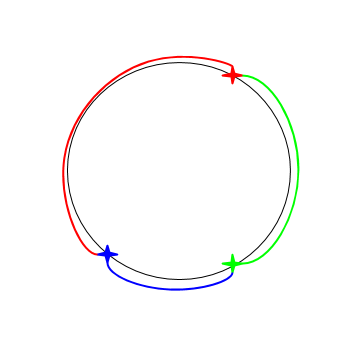
\includegraphics[width=0.5\linewidth]{figs/voro-chord-normal}
		\label{fig:voro-chord-normal}
	\end{figure}
	
\end{frame}

\note{Here, the nodes, the stars on this diagram are responsible for the region covered by the arc matching its color.  This repesents the space containing all keys greater than the ID of it's predecessor and less than or equal to its own ID.}

\begin{frame}{Chord Using A Different Closest Metric}
	\begin{figure}
		\centering
		\caption{A Voronoi diagram for a Chord network, where closest is defined by the node being the closest in either direction.}
		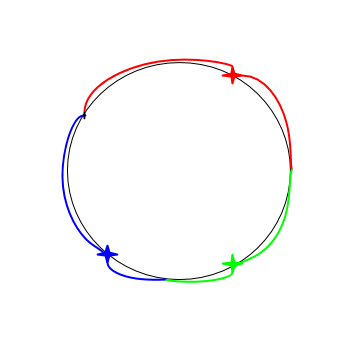
\includegraphics[width=0.5\linewidth]{figs/voro-chord-alternative}
		
		\label{fig:voro-chord-alternative}
	\end{figure}
\end{frame}


\note{In this figure, the ownership has the more intuitive definition of ``all points with to which I am the node with the shortest distance.''}


\begin{frame}{Terms and Variables}
	\begin{itemize}
		\item Network size is $n$ nodes.
		\item Keys and IDs are $m$ bit hashes, usually SHA1.
		\item Peerlists are made up of:
		\begin{description}
			\item[Short Peers] The neighboring nodes that define the network's topology.
			\item[Long Peers] Routing shortcuts.
		\end{description}
		\item We'll call the node responsible for a key the $ root $ of the key.
	\end{itemize}
\end{frame}

\note[itemize]{
	\item SHA1 is being depreciated, but this is trivial from our perspective.  
	\item Short peers are actively maintained, long peers replaced gradually and are not actively pinged.
	\item We use root as it's is a topology agnostic term.
}






\begin{frame}{Functions}
	\begin{description}
		\item[lookup($ key $)] Finds the node responsible for a given key.
		\item[put($ key $, $ value $)] Stores $value$ at the node responsible for $key$, where $key =  hash(value)$.
		\item[get($ key $)] Returns the $ value $ associated with $key$.
	\end{description}
\end{frame}

\note[itemize]{
	\item SPEED THRU THIS SLIDE
	\item These are the common function is every DHT:  lookup: find a node, put: store data, get: retrieve data.
	\item There is usually a delete function as well, but it's not important.
	\item All work the same way: if I can answer the function, great, otherwise return the node I know that's closest to the key, who will then do the same thing.
}





\subsection{Example DHT: Chord}

\begin{frame}{Chord}
	\begin{itemize}
		\item Ring Topology
		\item Short Peers: predecessor and successor in the ring.
		\item Responsible for keys between their predecessor and themselves.
		\item Long Peers:  $\log n$ nodes, where the node at index $i$ in the  peerlist is 
		$$ root(r + 2^{i-1} \mod  m) ,  1 < i  < m $$
		
		
		
	\end{itemize}
\end{frame}

\note[itemize]{
	\item Chord is a favorite because we can draw it.
	\item Draw a Chord network on the wall?
	\item node $r$ is our root node.
	\item $ i $ is the index on the list
	\item English for the equation, the long peers double in distance from the root node, allowing us to cover at least half the distance to our target in a step
	\item In this way, we can achieve an expected $ \lg n $  hops. 
}

\begin{frame}{A Chord Network}
	\begin{figure}
		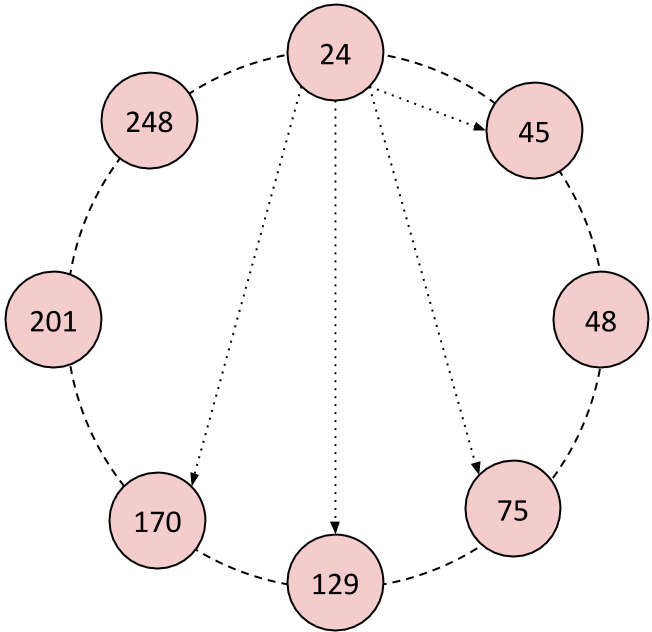
\includegraphics[width=0.55\linewidth]{figs/CR_overlay}
		\caption{An 8-node Chord ring where $m=8$.  Node 24's long peers are shown.}
		\label{fig:chordreal}
	\end{figure}
\end{frame}

\note[itemize]{
	\item The dashed lines are the short links; each node keeps track of its successor and predecessor.
	\item The dotted lines are node 24's long links; since $ m = 8$  there's 8, but since the network is so small,  4 are duplicates.
	\item Traffic travels clockwise.
	}

\begin{frame}{Fault Tolerence in Chord}
	\begin{itemize}
		\item Local maintenance thread  gradually fixes the network topology.
		\begin{itemize}
			\item Each node ``notifies'' its successor.
			\item The successor replies with a better successor if one exists.
		\end{itemize}
		\item The long peers are gradually updated by performing a lookup on each entry.
		
	\end{itemize}
\end{frame}

\note[itemize]{
	\item The notification allows a sucessor to either update its predecessor if incorrect and the predecessor to update its successor if wrong
	\item Some implementations use predecessor and successor lists.
	\item The long peers are replaced much slower; maintenance slowly iterates through the long peers and queries to see if there's better node for that particular long peer.
}

\begin{frame}{Handling Churn in General}
	\begin{itemize}
		\item Short peers, the neighbors, are periodically queried to:
		\begin{itemize}
			\item See of the node is still alive.
			\item See if the neighbor knows about better nodes.
		\end{itemize}
		\item Long peer failures are replaced by regular maintenance.
	\end{itemize}
\end{frame}


\note[itemize]{
	\item Short peers need to be actively maintained to keep the topology correct.
	\item	
}
%\subsection{Other DHTs}
%\begin{frame}{Other DHTs}
%	Other DHTs include
%	\begin{itemize}
%		\item Kademlia 
%		\item Pastry and Tapestry
%		\item CAN
%		\item Symphony %
%		\item ZHT
%	\end{itemize}
%\end{frame}

\section{Completed Work}



\begin{frame}{Overarching Goal}
My research has been focused on:
	\begin{itemize}
		\item Abstracting out DHTs.
		\item Distributed computation using DHTs.
	\end{itemize}
\end{frame}

\note[itemize]{
	\item I want to get down to what the essence of a DHT is, find out what all DHTs have in common, so that I could create a generic DHT.
	\item I focused on creating a more abstract framework for MapReduce, so I could move it out of the datacenter and into other contexts.
	\item We'll first discuss generalizing DHTs.
}


\subsection{VHash}



\begin{frame}{Goals}
	VHash sprung from two related ideas:
	\begin{itemize}
		
		\item<1-> We wanted a way be able optimize latency by embedding it into the routing overlay. \note<1>{Most DHTs optimize routing for the number of hops, rather than latency.}
		\item<2-> We wanted to create a DHT based off of Voronoi tessellations. Unfortunately: \note<2>{ We discovered a mapping between Distributed Hash Tables and Voronoi/Delaunay Triangulations.}
		\begin{itemize}
			\item<3-> Distributed algorithms for this problem don't really exist.  \note<3>{I lie, they do exist, but they all are ``run the global algorithm on your local subset.  And if we move out of or above 2D Euclidean space, as Brendan wanted to, no fast algorithms exist at all.  We quickly determined that solving was never really a feasible option. So that leaves approximation.  A distributed algorithm would be helpful for some WSNs solving the boundary coverage problem.}
			\item<4-> Existing approximation algorithms were unsuitable. \note<4>{Simple approximations have no guarantees of connectivity, which is very bad for a routing topology.  Better algorithms that existed for this problem technically ran in constant time, but had a prohibitively high sampling.  So to understand what I'm talking about here, let's briefly define what a Voronoi tessellation is.}
		\end{itemize}
		%		\item<5>  We wanted to the nodes to move in the key space to adjust to . \note{Just a minor challenge no }
	\end{itemize}
\end{frame}


\begin{frame}{Voronoi Tesselation}
	\begin{figure}
		\centering
		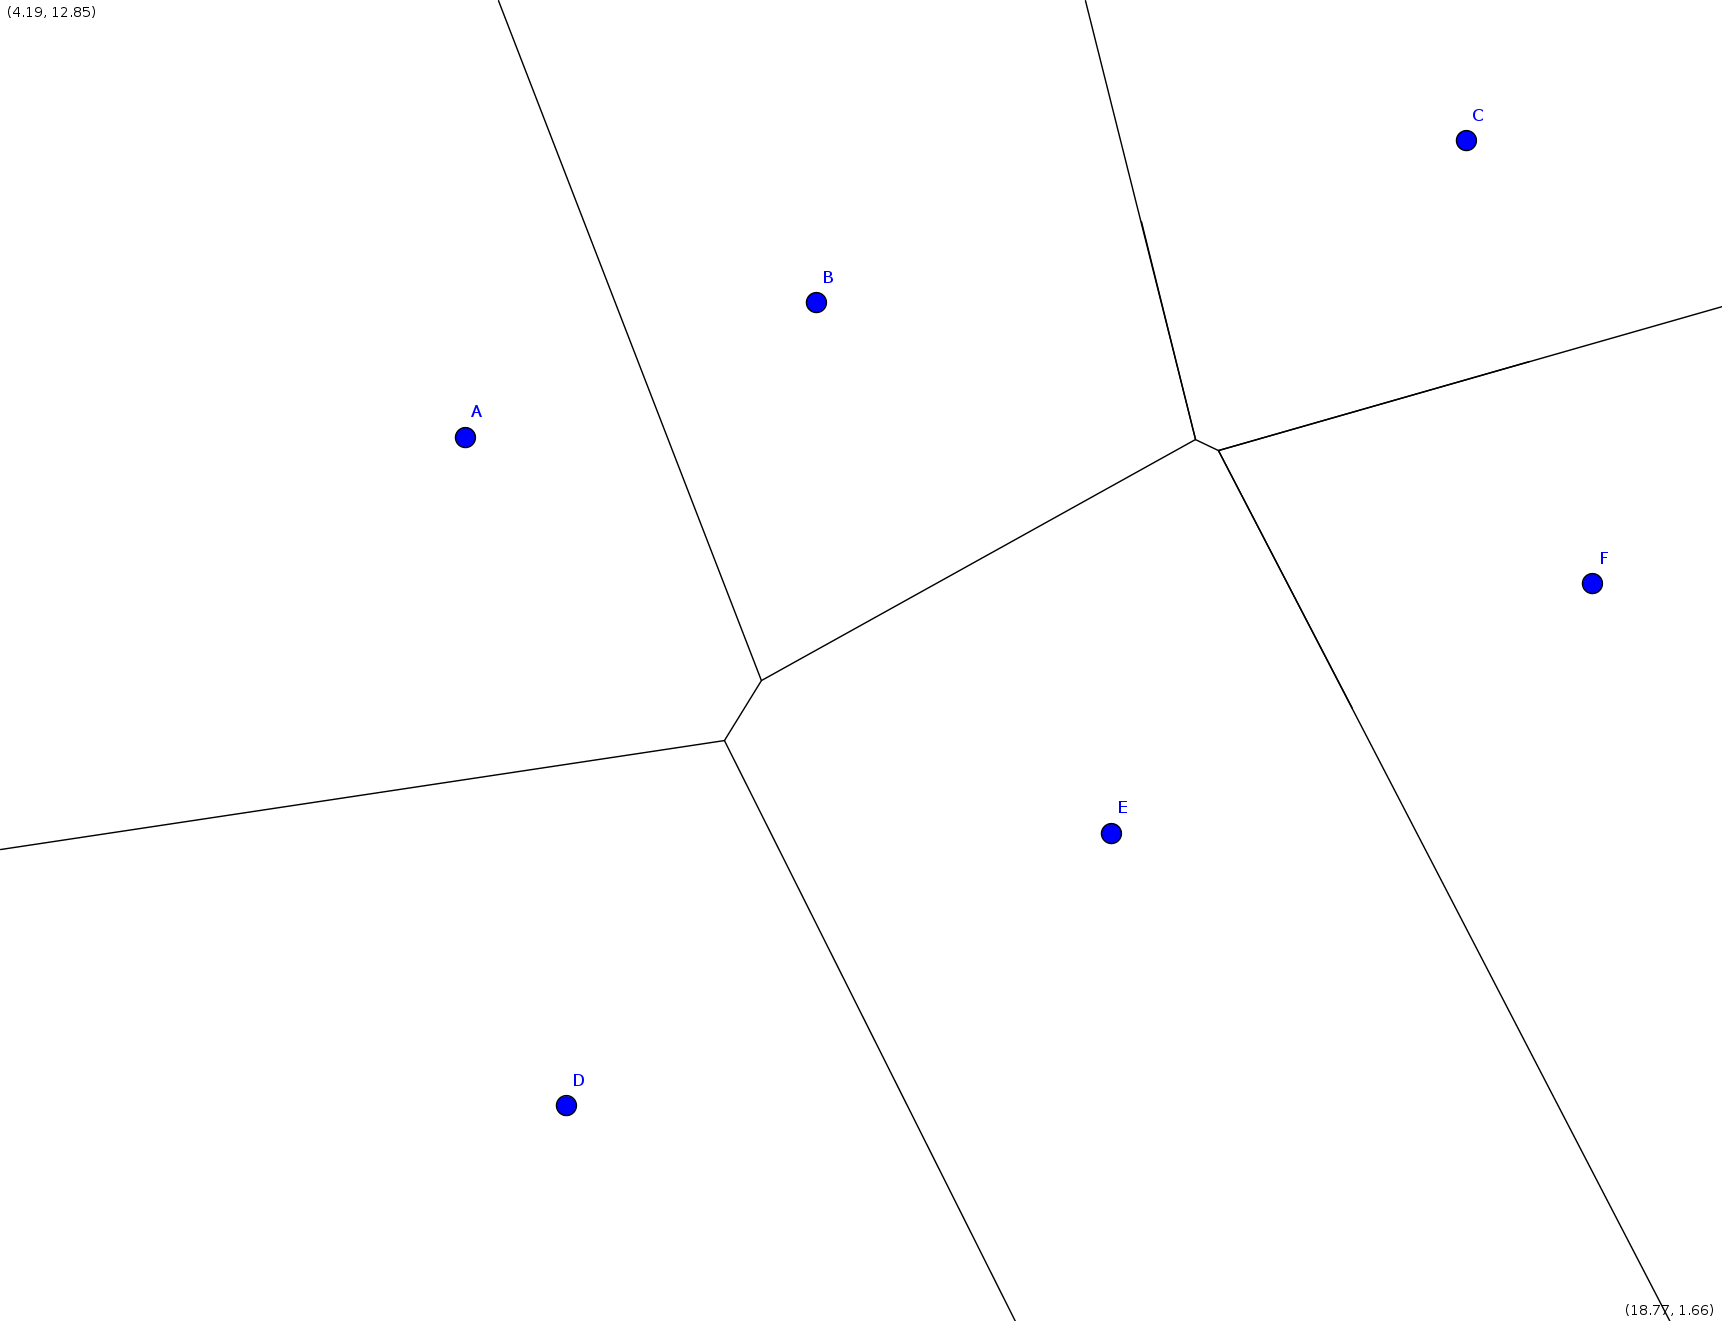
\includegraphics[width=0.5\linewidth]{figs/new_voronoi}
		\caption{A set of points and the generated Voronoi regions}
		\label{fig:new_voronoi}
	\end{figure}
\end{frame}

\note{Define
	\begin{itemize}
		\item A Voronoi tessellation or Voronoi diagram divides a space into regions, where each region encompasses all the points closest to Voronoi generators (point).
		\item Voronoi generators
		\item Voronoi Region
		\item Voronoi Tessellation/ Diagram
	\end{itemize}
}

\begin{frame}{Delaunay Triangulation}
	\begin{figure}
		\centering
		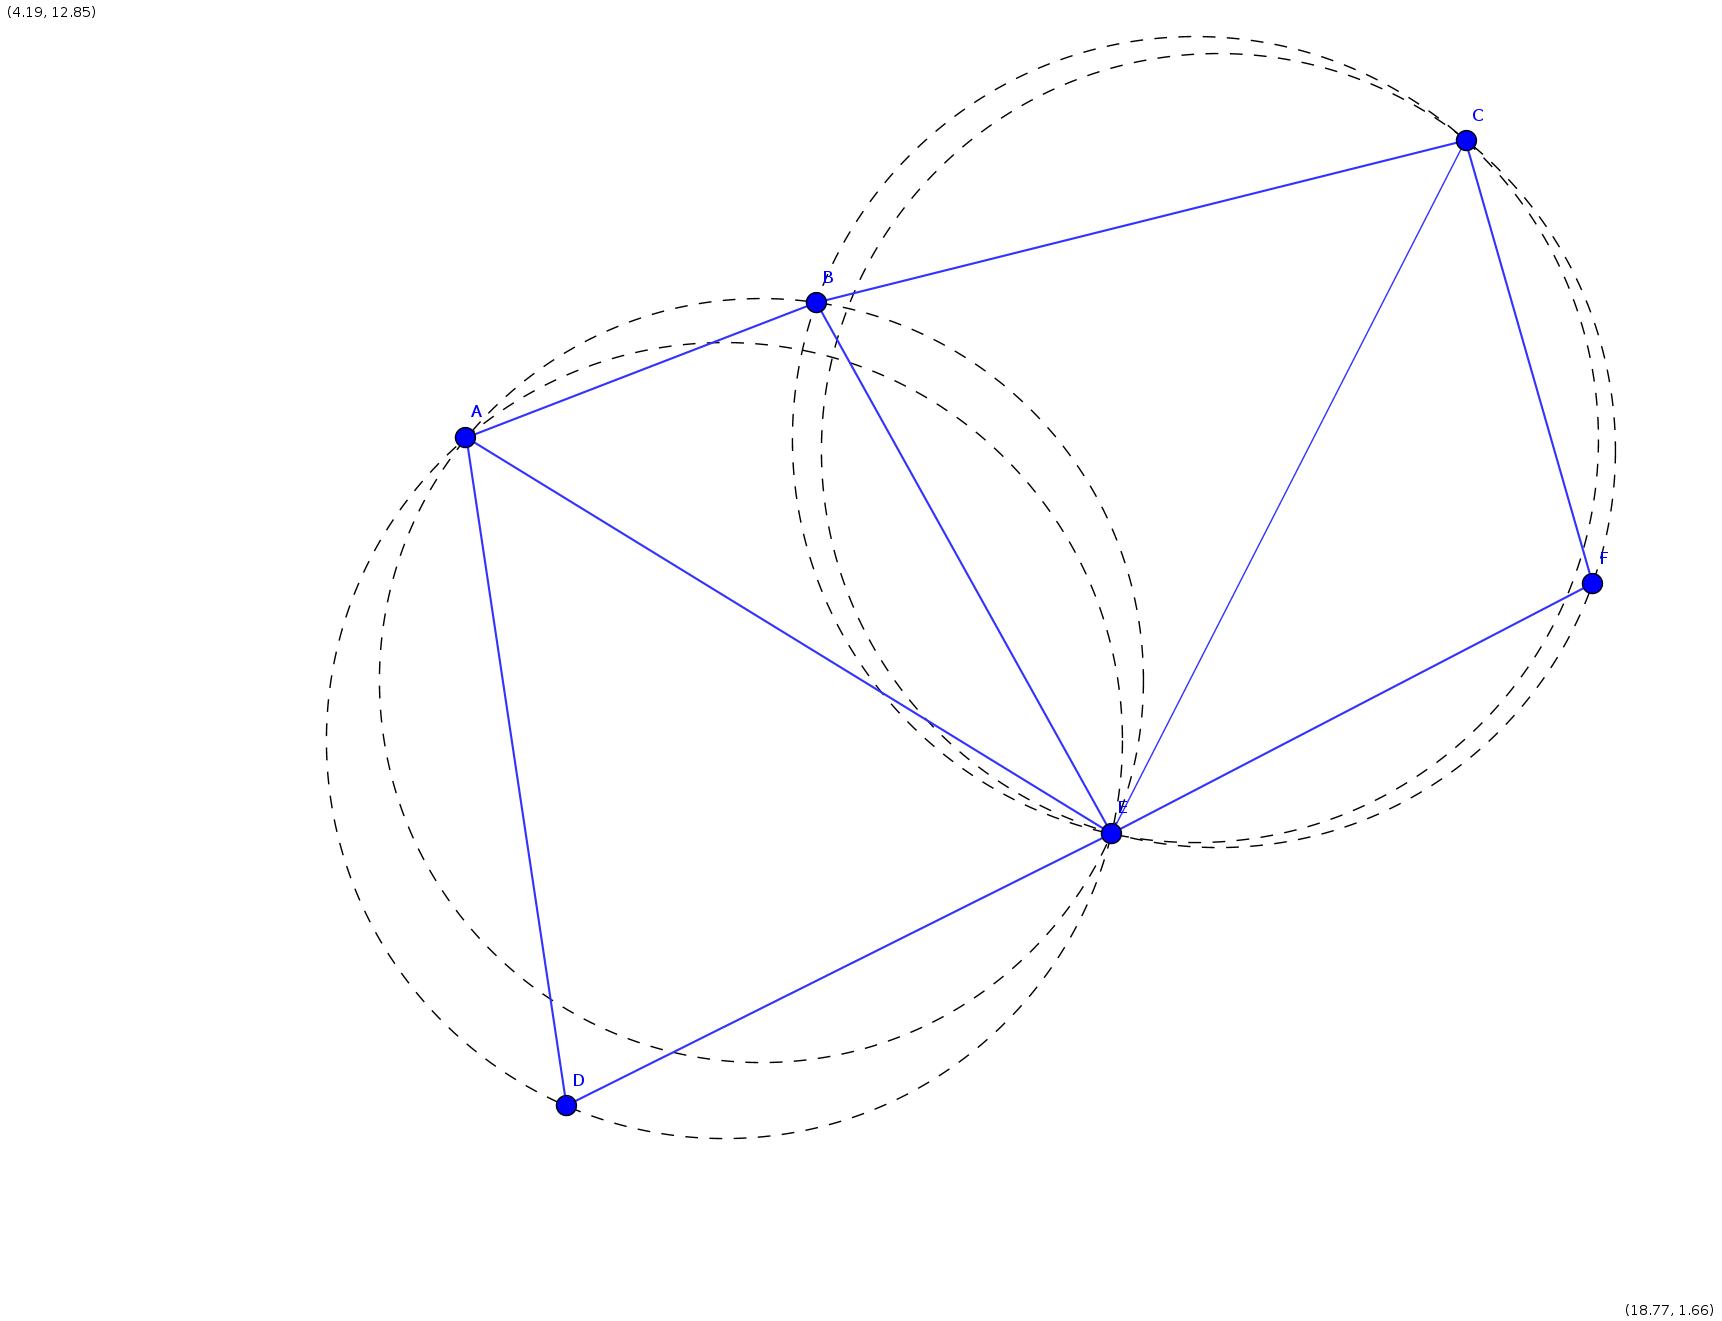
\includegraphics[width=0.5\linewidth]{figs/delaunay}
		\caption{The same set of nodes with their corresponding Delaunay Triangulation.}
		\label{fig:delaunay}
	\end{figure}
\end{frame}

\note{Define
	\begin{itemize}
		\item Delaunay Triangulation is a triangulation of a set of points with the following rule:
		\item No point falls within any of the circumcirles for every triangle in the triangulation, 
		\item The Voronoi tessellation and Delaunay Triangulation are dual problems
		\begin{itemize}
			\item Solving one yields the other.
			\item We can get the Voronoi diagram by connecting all the centers of circumcircles.
			\item 
		\end{itemize}
	\end{itemize}
}


\begin{frame}{DHT and Voronoi Relationship }
	\begin{itemize}
		\item We can view DHTs in terms of Voronoi tessellation and Delaunay triangulation.
		\begin{itemize}
			\item The set of keys the node is responsible for is its Voronoi region.
			\item The nodes neighbors are it's Delaunay neighbors.
		\end{itemize}
	\end{itemize}
\end{frame}

\note{
	It turns out we  can look at distributed hash tables in terms of Voronoi tessellation and Delaunay triangulation. 
	So if we have a quick way approximate this, we can build a DHT based directly on Voronoi tessellation and Delaunay triangulation.
}

\begin{frame}{VHash}
	\begin{itemize}
		\item Voronoi-based Distributed Hash Table based on this relationship.
		\item Uses our approximation to solve for Delaunay neighbors, called DGVH.
		\item Topology updates occur via  gossip-based protocol. 
		\item Routing speed is $ O(\sqrt[d]{n} ) $
		\item Memory Cost
		\begin{itemize}
			\item Worst case: $O(n)$
			\item Expected maximum size: $\Theta(\frac{\log n}{\log \log n} )$
		\end{itemize}
	\end{itemize}
\end{frame}

\note[itemize]{
	\item Gossip:  every cycle, a node chooses a peer and swaps peerlist information, then reruns the approximation.
	\item $d$ is number of dimensions, but we optimize over latency so that's deceptive
	\item This would only happen in a contrived case and would give $ O(1) $ routing
	\item We found a paper that proved $\Theta(\frac{\log n}{\log \log n} )$  is the expected maximum degree of a vertex in a Delaunay Triangulation.
}

\begin{frame}{Distributed Greedy Voronoi Heuristic}
	
	\begin{itemize}
		\item Assumption: The majority of Delaunay links cross the corresponding Voronoi edges.
		\item We can test if the midpoint between two potentially connecting nodes is on the edge of the Voronoi region.
		\item This intuition fails if the midpoint between two nodes does not fall on their Voronoi edge.
	\end{itemize}
	
\end{frame}

\begin{frame}{DGVH Heuristic}
	
	\begin{algorithmic}[1]  % the numberis how many lines
		\STATE Given node $n$ and its list of $candidates$.
		\STATE $peers \leftarrow$ empty set that will contain $n$'s one-hop peers
		\STATE Sort $candidates$ in ascending order by each node's distance to $n$
		\STATE Remove the first member of $candidates$ and add it to $peers$
		\FORALL{$c$ in $candidates$}
		\STATE $m$ is the midpoint between $n$ and $c$
		\IF{Any node in $peers$ is closer to $m$ than $n$}
		\STATE Reject $c$ as a peer
		\ELSE
		\STATE Remove $c$ from $candidates$
		\STATE Add $c$ to $peers$
		\ENDIF
		\ENDFOR
	\end{algorithmic}
	
\end{frame}



\note{
	\begin{enumerate}
		\item 'n' is the "myself" node, and the location we are seeking to find the peers of.
		\item  peers is a set that will build the peerlist in
		\item We sort the candidates from closest to farthest.
		\item The closest candidate is always guaranteed to be a peer.
		\item Iterate through the sorted list of candidates and either add them to the peers set or discard them.
		\item We calculate the midpoint between the candidate and the center 'n'. 
		\item If this midpoint is closer to a peer than 'n', then it does not fall on the interface between the location's Voronoi regions.
		\item in this case discard it
		\item otherwise add it the current peerlist
	\end{enumerate}
}


\note{
	DVGH is very efficient in terms of both space and time.
	Suppose a node $n$ is creating its short peer list from $k$ candidates in an overlay network of $N$ nodes.
	The candidates must be sorted, which takes $O(k\cdot\lg(k))$ operations.
	Node $n$ must then compute the midpoint between itself and each of the $k$ candidates.
	Node $n$ then compares distances to the midpoints between itself and all the candidates.
	This results in a cost of
	
	\[ k\cdot\lg(k) + k \text{ midpoints}  + k^{2} \text{ distances} \]
	
	
	Since $k$ is  bounded by $\Theta(\frac{\log N}{\log \log N} )$ (the expected maximum degree of a node), we can translate the above to
	
	\[O(\frac{\log^{2} N}{\log^{2} \log N} )\]
	
	In the vast majority of cases, the number of peers is equal to the minimum size of \textit{Short Peers}.
	This yields $k=(3d+1)^{2}+3d+1$ in the expected case, where the lower bound and expected complexities are $\Omega(1)$.
}



\begin{frame}{Results}
	\begin{figure}
		\centering
		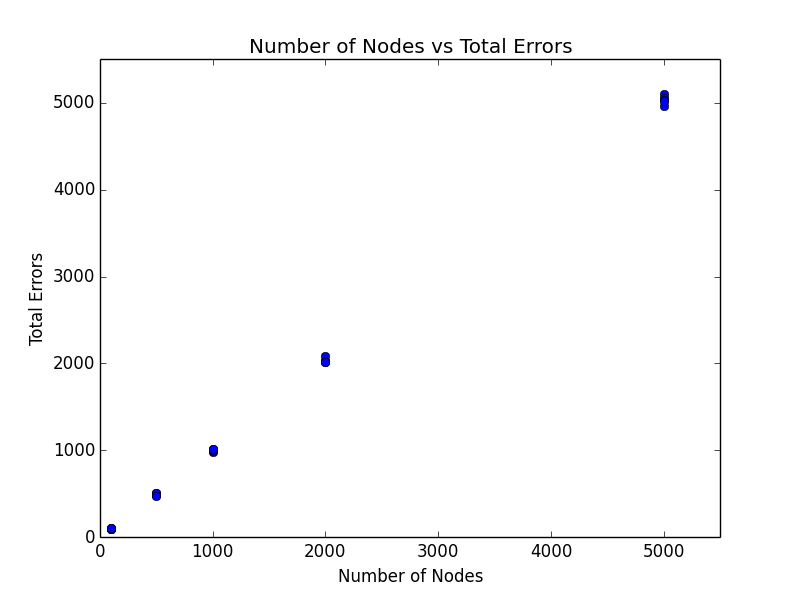
\includegraphics[width=0.75\linewidth]{figs/error_rate}
		\caption{As the size of the graph increases, we see approximately 1 error per node.
%			We can also see that the error rate and number of nodes has a linear relationship.
			}
		\label{exp_0}
	\end{figure}
\end{frame}

\note[itemize]{
	
	\item The error is approximately 1 missed delaunay neighbor per node, so the entire generated mesh is a subset of the true delaunay trinagulation.
	\item This error is acceptable since we miss an edge when it is occluded by another node in the way.
	}

\begin{frame}{Results}
	\begin{figure}
		\label{fig:conv}
		\centering
		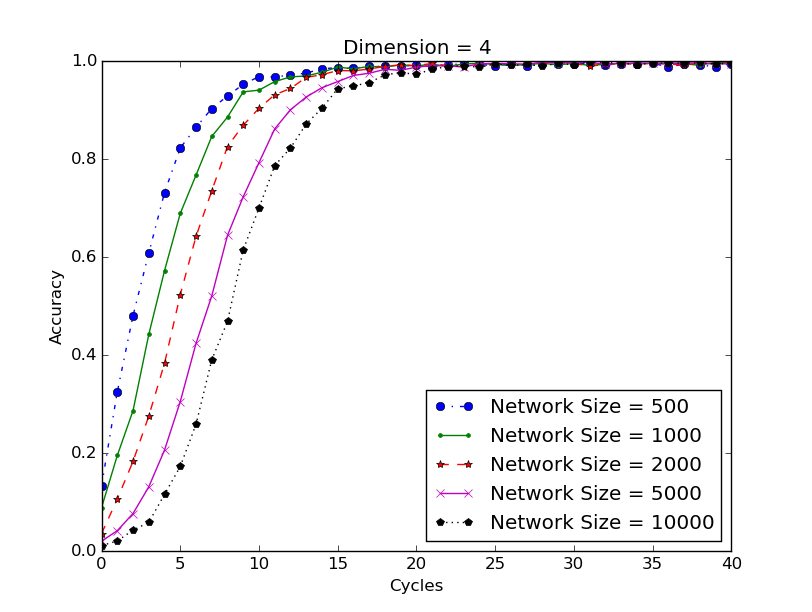
\includegraphics[width=0.75\linewidth]{figs/conv_d4}
		%\caption{This plot shows the accuracy rate of lookups on a 4-dimensional network as it self-organizes.}
		\label{conv4}
	
		\caption{These figures show, starting from a randomized network, VHash forms a stable and consistent network topology. %The Y axis is the percentage of successful lookups out of 2000 queries and the X axis is the number of gossips cycles.}
		}
		
	\end{figure}
\end{frame}

\note[itemize]{
	\item Our first experiment was to confirm that VHash creates a stable mesh.

	}

\begin{frame}{Results}
	\begin{figure}
		
		\centering
		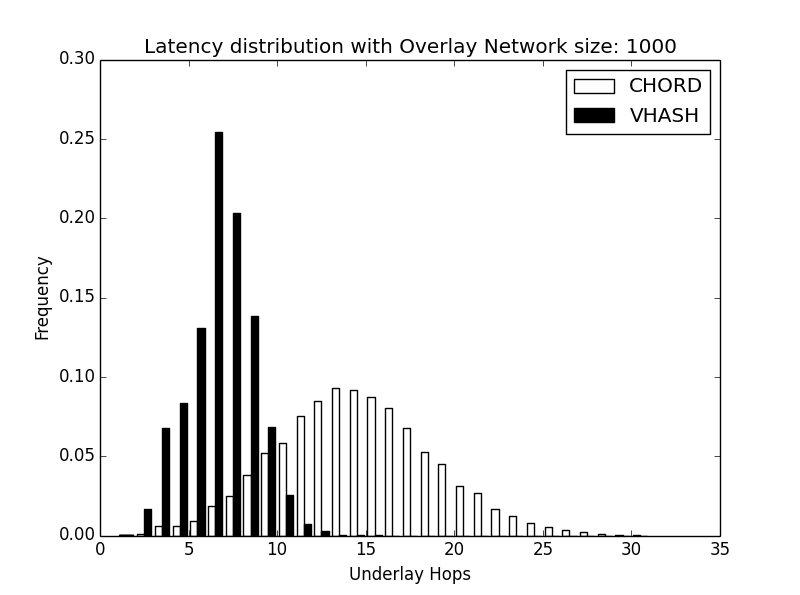
\includegraphics[width=0.75\linewidth]{figs/hist_1000}
		\caption{Comparing the routing effectiveness of Chord and VHash.}
		\label{fig:hist1000}
	\end{figure}
	
\end{frame}

\note[itemize]{
	\item For this experiment, we constructed a scale free network with 10000 nodes placed at random (which has an approximate diameter of 3 hops) as an underlay network .
	\item scale free networks model the Internet's topology.
	\item We then chose a random subset of nodes to be members of the overlay network.
	\item We then measured the distance in underlay hops between 10000 random source-destination pairs in the overlay.
	\item VHash generated an embedding of the latency graph utilizing a distributed force directed model, with the latency function defined as the number of underlay hops between it and its peers.
	
	
	\item This how the difference in the performance of Chord and VHash for 10,000 routing samples on a 10,000 node underlay network for differently sized overlays.
	The Y axis shows the observed frequencies and the X axis shows the number of hops traversed on the underlay network.
	VHash consistently requires fewer hops for routing than Chord.
	
}

\begin{frame}{Conclusions}
	\begin{itemize}
		\item DGVH is simple approximation for Delaunay Triangulation that guarantees a fully connected graph.
		\item VHash can optimize over a metric such as latency and achieve superior routing speeds as a result.
	\end{itemize}
\end{frame}		

\note[itemize]{
	\item DGVH is of similar complexity to picking $k$-nearest node or nodes in distance $k$.
	\item other methods don't guarantee full connectivity
	\item It caps out at $O(n^2)$ complexity, no matter how many dimensions or complexities of the metric space (unless calculating distance or midpoint is worse than $O(1)$)
	\item for example This means you can use in it an 100-dimensional euclidean space in $O(n^2)$ time rather than $O(n^{50})$ time (maybe we should have opened with this...)
}





\subsection{ChordReduce}

\begin{frame}{Goals}

	\begin{itemize}
		\item We wanted build a more abstract system for MapReduce.
		\item We remove core assumptions:
		\begin{itemize}
			\item The system is centralized.
			\item Processing occurs in a static network.
		\end{itemize}
		\item The resulting system must be:
		\begin{itemize}
			\item Completely decentralized.
			\item Scalable.
			\item Fault tolerant.
			\item Load Balancing.
		\end{itemize}
	\end{itemize}

\end{frame}


%
%\begin{frame}{System Architecture}  %
%	ChordReduce has three layers:
%	\begin{itemize}
%		\item Chord \cite{Chord}, which handles routing and lookup.
%		\item The Cooperative File System (CFS) \cite{CFS}, which handles storage and data replication.
%		\item The MapReduce layer.
%	\end{itemize}
%
%\end{frame}
%

\begin{frame}{System Architecture}
	\begin{figure}
	    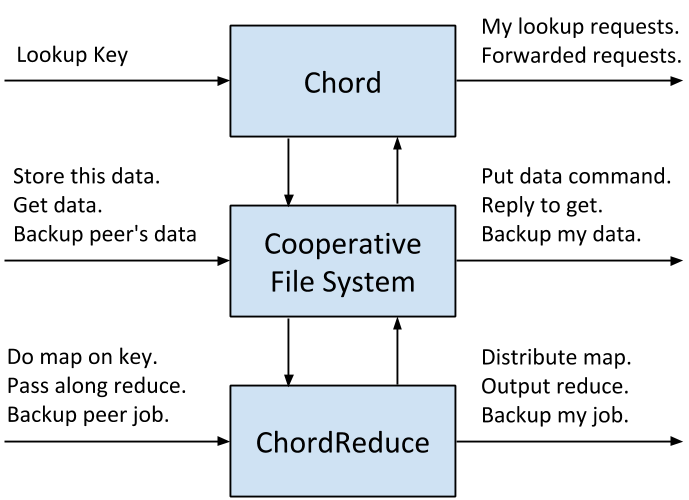
\includegraphics[width=0.8\linewidth]{figs/CR_architecture}
	
	\end{figure}
\end{frame}



\note[itemize]{
		\item Chord, which handles routing and lookup.
		\item The Cooperative File System (CFS), which handles storage and data replication.
		\item The MapReduce layer.

		\item Files are split up, each block given a key based on their contents.
		\item Each block is stored according to their key.
		\item The hashing process guarantees that the keys are distributed near evenly among nodes.
		\item A keyfile is created and stored where the whole file would have been found.
		\item To retrieve a file, the node gets the keyfile and sends a request for each block listed in the keyfile	
}


\begin{frame}{Mapping Data}
	\begin{figure}
	    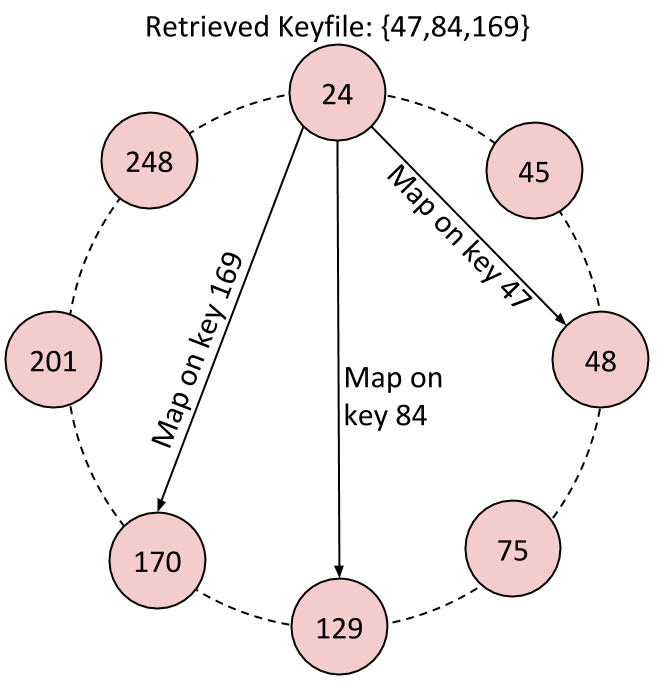
\includegraphics[width=0.48\linewidth]{figs/CR_dataflow2}
	    \caption{ \footnotesize{The stager sends a map task for each key in the keyfile. In larger networks, this process is streamlined by recursively bundling keys and sending them to the best finger.}}
		
	\end{figure}
\end{frame}


\note[itemize]{
\item this process is recursive
}


\begin{frame}{Reducing Results of Data}
	\begin{figure}
	    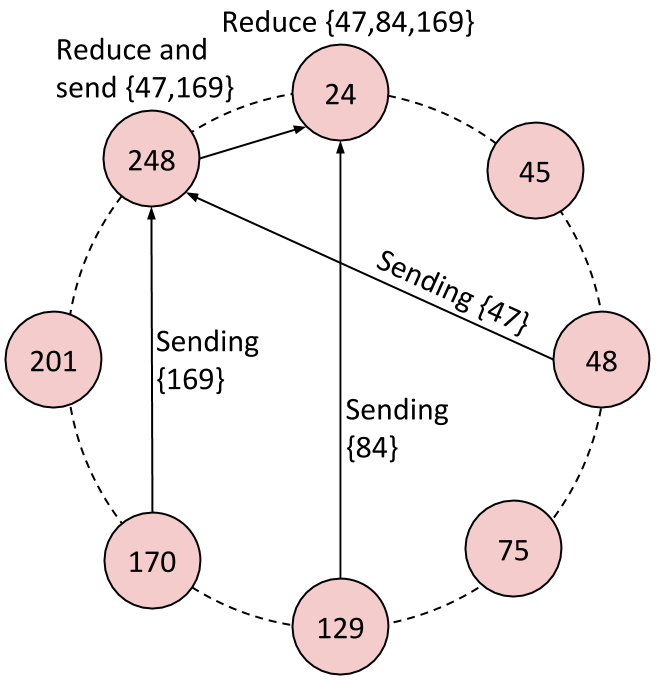
\includegraphics[width=0.50\linewidth]{figs/CR_dataflow3}
	    \caption{Results are sent back via the overlay. If a node receives multiple results, they are reduced before being sent on.}
	\end{figure}
\end{frame}

\note{The paths here are arbitrary edges that I came up with for the example.}


\begin{frame}{Experiment Details}
	Our test was a Monte Carlo approximation of $\pi$.
	\begin{columns}[T]
	
	
		\begin{column}{.5\textwidth}
		
			\begin{figure}
			    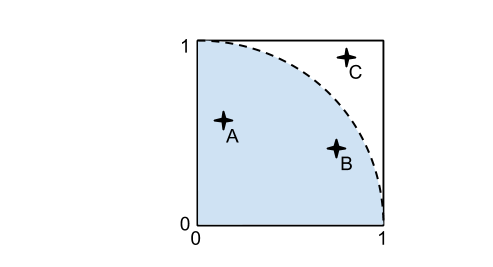
\includegraphics[width=\linewidth]{figs/dartboard}
			    \caption{The node chooses random $x$ and $y$ between 0 and 1. If $x^{2} + y^{2} < 1^{2} $, the ``dart ''landed inside the circle.}
			    \label{dartboard}
			\end{figure}
			
			
		\end{column}
			
		\begin{column}{.5\textwidth}
			\begin{itemize}
				\item Map jobs were sent to randomly generated hash addresses.
				\item The ratio of hits to generated results approximates $\frac{\pi}{4}$.
				\item Reducing the results was a matter of combining the two fields.
			\end{itemize}
		\end{column}
		
	\end{columns}
\end{frame}


\note[itemize]{
\item Experiment had these goals
\begin{enumerate}
	\item ChordReduce provided significant speedup during a distributed job.
	\item ChordReduce scaled.
	\item ChordReduce handled churn during execution.
\end{enumerate}
}

\begin{frame}{Experimental Results}

	\begin{figure}
	    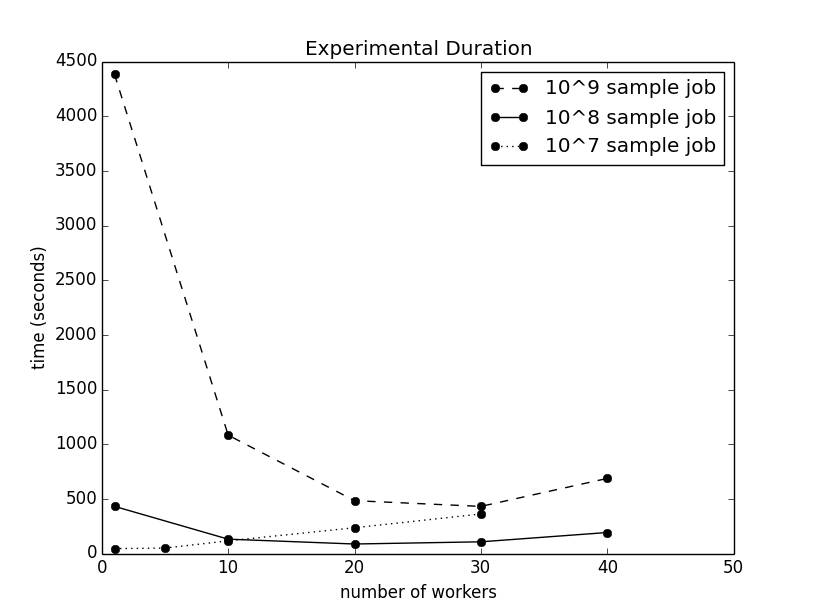
\includegraphics[width=0.75\linewidth]{figs/expTime}
	    \caption{For a sufficiently large job, it was almost always preferable to distribute it.}
	    \label{expTime}
	\end{figure}


\end{frame}
\note[itemize]{
	\item When the job is too small, such as with the $10^{7}$ data set, our runtime is dominated by the overhead.  
	\item Our results are what we would expect when overhead grows logarithmically to the number of workers.
	\item Diminishing returns.

}



\begin{frame}{Churn Results}
	\begin{table}
		\centering
		\begin{tabular}{|r|r|r|} 
			\hline 
			Churn rate per second & Average runtime (s) & Speedup vs 0\% churn\\ \hline{}
			0.8\% & 191.25 & 2.15 \\ \hline
			0.4\% & 329.20 & 1.25 \\ \hline
			0.025\% & 431.86 & 0.95 \\ \hline 
			0.00775\%  & 445.47 & 0.92 \\ \hline 
			0.00250\% & 331.80  &  1.24 \\ \hline 
			0\% & 441.57 & 1.00 \\ \hline
		\end{tabular}
		\caption{The results of calculating $\pi$ by generating $10^8$ samples under churn. Churn is the chance for each node to join or leave the network. The large speedup is from joining nodes acquiring work during experimental runtime.} 
		\label{tab:churnSpeed}
	\end{table}
	
\end{frame}

\note[itemize]{
	\item We tested at rates from 0.0025\% to 0.8\% \textbf{\textit{per second}}, 120 times the fastest rate used to test P2P-MapReduce.
	
	\item ChordReduce finished twice as fast under the unrealistic levels churn (0.8\% per second) than no churn (Table \ref{tab:churnSpeed}).
	
	\item Churn is a disruptive force; how can it be aiding the network?  We have two hypotheses
	\item Deleting nodes motivates other nodes to work harder to avoid deletion (a ``beatings will continue until morale improves'' situation).
	\item Our high rate of churn was dynamically load-balancing the network.  How?
	\item Nodes that die and rejoin are more likely to join a region owned by a node with larger region and therefore more work.
	\item It appears even the smallest effort of trying to dynamically load balance, such as rebooting random nodes to new locations, has benefits for runtime.
		Our method is a poor approximation of dynamic load-balancing, and it still shows improvement.
	
}


\begin{frame}{Conclusions}
Our experiments established:
\begin{itemize}
	\item ChordReduce can operate under high rates of churn.
	\item Execution follows the desired speedup.
	\item Speedup occurs on sufficiently large problem sizes.
\end{itemize}

This makes ChordReduce an excellent platform for distributed and concurrent programming in cloud and loosely coupled environments.

\end{frame}

\note{
	One of the goals coming out of this is that I want to be able to harness this speedup due to churn.  I've come up with a number of potential strategies I've listed in the proposal, but a number of them involve nodes being able to create virtual nodes, in other words, be in multiples places at once and have multiple identities.
	
	It turns out the security world has something analogous to that.
}

\subsection{Sybil Attack Analysis}

\begin{frame}{The Sybil Attack}
	\begin{itemize}
		\item The Sybil attack is a type of attack against a distributed system such as a DHT.
		\item The adversary pretends to be more than one identity in the network.
		\begin{itemize}
			\item Each of these false identities, called a \alert{Sybil} is treated as a full member of the network.
		\end{itemize}
		\item The overall goal is to occlude healthy nodes from one another.
		\item The Sybil attack is extremely well known, but there is little literature written from the attacker's perspective.
	\end{itemize}
	
\end{frame}

\note[itemize]{
	\item DHTs don't have a centralized point of failure, but this opens up different strategies for attack
	\item How the identities are obtained is a question for later, but we assume they don't have to be real hardware.
	\item By occlude, we me that that traffic must travel thru the adversary.
	\item What distinguishes the Sybil from the Eclipse attack is the fact that the Sybil attack relies only on false identity
}


\begin{frame}
	\frametitle{The Sybil Attack in A P2P network}
	See Whiteboard
	\begin{itemize}
		\item We want to inject a Sybil into as many of the regions between nodes as we can.
		\item The question we wanted to answer is what is the probability that a region can have a Sybil injected into it, given:
		\begin{itemize}
			\item The network size $n$
			\item The number of IDs available to the attacker (the number of identities they can fake).
		\end{itemize}
	\end{itemize}
	\end{frame} 
       
\begin{frame}
\frametitle{Assumptions}
	\begin{itemize}
		\item The attacker is limited in the number of identities they can fake.		
		\begin{itemize}
			\item To fake an identity, the attacker must be able to generate a valid IP/port combo he owns.
			\item The attacker therefore has $num\_IP \cdot num\_ports$ IDs.
			\item We'll set $ num\_ports = 16383 $, the number of ephemeral ports.
			\item Storage cost is 320 KiB.
		\end{itemize}
		\item We call the act of finding an ID by modulating your IP and port so you can inject a node \emph{mashing}.
		\item In Mainline DHT, used by BitTorrent, you can choose your own ID at ``random.''   The implications should be apparent.
	
	\end{itemize}
\end{frame}

\begin{frame}
    \frametitle{Analysis}
    The probability you can mash a region between two adjacent nodes in a size $n$ network is:
     \begin{equation}
    P \approx \frac{1}{n}\cdot num\_ips \cdot num\_ports
    \end{equation}
    An attacker can compromise a portion $ P_{bad\_neighbor} $ of the network given by:
    \begin{equation}
    P_{bad\_neighbor} =  \frac{num\_ips \cdot num\_ports}{num\_ips \cdot num\_ports + n - 1}
    \label{eq:bad}
    \end{equation}
    
\end{frame}
\note[itemize]{\item Have proofs!}


\begin{frame}
    \begin{figure}
        \centering
        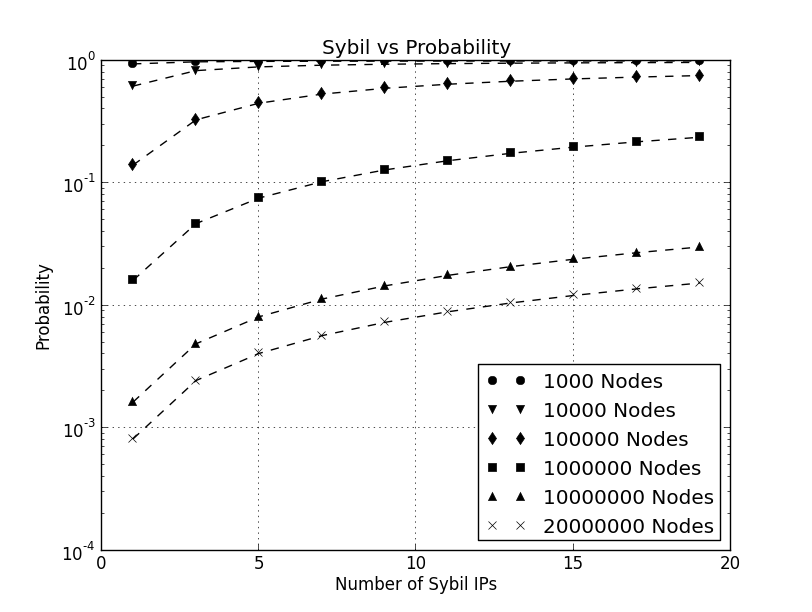
\includegraphics[width=0.75\linewidth]{figs/ip_prob_all}
        \caption[foo]{Our simulation results.  
           
            The dotted line traces the line corresponding to the Equation \ref{eq:bad}: $ P_{bad\_neighbor} =  \frac{num\_ips \cdot 16383}{num\_ips \cdot 16383 + n - 1}$}.
        \label{fig:exp2}
    \end{figure}
\end{frame}
\note{ The $x$-axis corresponds to the number of IP addresses the adversary can bring to bear.
	The $y$-axis is the probability that a random region between two adjacent normal members of the network can be mashed.
	Each line maps to a different network size of $n$.}


\begin{frame}
    
    \begin{figure}
        \centering
        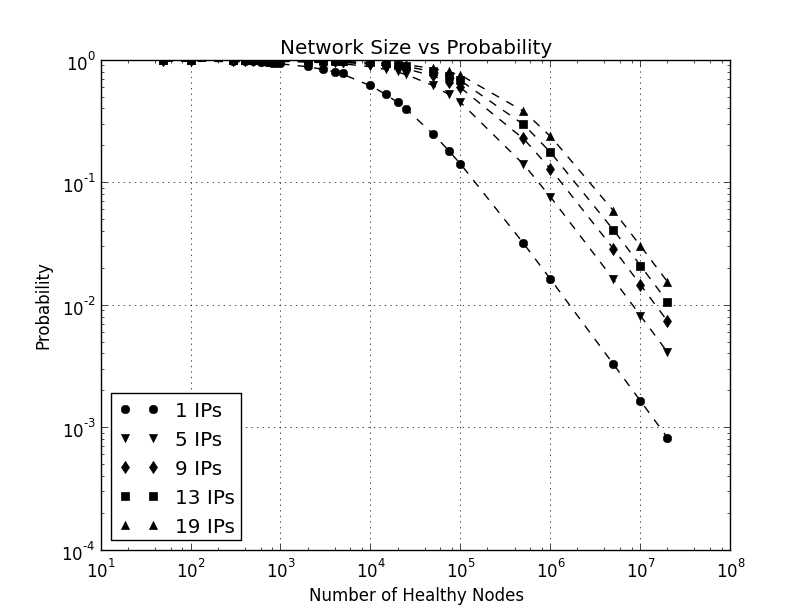
\includegraphics[width=0.75\linewidth]{figs/size_prob_all}
        \caption[a]{These are the same as results shown in Figure \ref{fig:exp2}, but our $x$-axis is the network size $n$ in this case.  
            Here, each line corresponds to a different number of unique IP addresses the adversary has at their disposal.}
        \label{fig:size_prob_all}
    \end{figure}
\end{frame}

\begin{frame}
    \begin{figure}
        \centering
        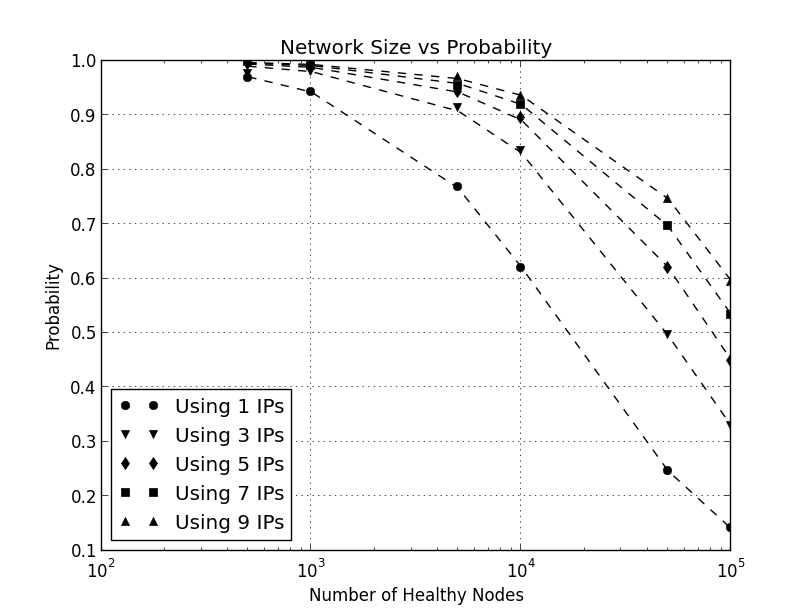
\includegraphics[width=0.7\linewidth]{figs/size_occlusion_chord}
        \caption{This graph shows the relationship between the network size and the probability a particular link, adjacent or not, can be mashed.}
        \label{fig:exp3}
    \end{figure}
\end{frame}
    
\begin{frame}{Conclusion}
	\begin{itemize}
		
		\item Our analysis showed an adversary with limited resources can occlude the majority of the paths between nodes.
		\item An attack of this sort on Mainline DHT would cost about \$43.26 USD per hour.
		\item Moreover, we demonstrated that creating virtual nodes is cheap and easy.
	\end{itemize}
\end{frame}

\note[itemize]{
	\item By cost, that is the Amazon EC2 cost and assumed half the links of 20,000,000 nodes we occluded.
}

\section{Proposed Work}



\subsection{UrDHT}
\begin{frame}{UrDHT}
	\begin{itemize}
		\item UrDHT is a completely abstracted DHT that will serve as a framework for creating DHTs.
		\item The goal is \textbf{not only} to create a DHT, but to create an easily extensible abstract framework for DHTs.
		\item Continuation of the work in VHash.
	\end{itemize}
\end{frame}


\note[itemize]{
	\item \textit{Ur} as in the germanic prefix for proto or first
	\item UrDHT is a project that presents a minimal and extensible implementation for all the essential components for a DHT: the different aspects for a protocol definition, the storage of values, and the networking components.
	Every DHT has the same components, but there has yet to be an all-encompassing framework that clearly demonstrates this.
}

\begin{frame}{UrDHT}
	\begin{itemize}
		\item We will be creating a mathematical description of what a DHT is.
		\item We will implement various DHTs using UrDHT and compare their performance.

	\end{itemize}
\end{frame}



\note[itemize]{
	\item The purpose of doing this is that
	\item it's cool
	\item We want a framework for creating DHTs and DHT based applications to be easily available
	\item I need it to do the rest of my proposal and Brendan needs it for the same reason.
}


\subsection{DHT Distributed Computing}
\begin{frame}{DHT Distributed Computing}
	\begin{itemize}
			\item We will use UrDHT to implement a few of the more popular DHTs.
			\begin{itemize}
				\item See if there is a difference for distributed computing.
				\item Using UrDHT for all the implementations will minimize the differences between each DHT.	
			\end{itemize}
		
	\end{itemize}
\end{frame}
\note[itemize]{
	\item Additionally this will serve as an example of how to implement our framework. 
}


\begin{frame}{DHT Distributed Computing}
	\begin{itemize}
			\item Implement distributed computing on each of the implemented DHTs.
			\begin{itemize}
				\item The emphasis is robustness and fault-tolerance.
			\end{itemize}
			\item Test each framework using a variety of embarrassingly parallel problems, such as:
			\begin{itemize}
				\item Brute-force cryptanalysis.
				\item MapReduce problems.
				\item Monte-Carlo computations.
			\end{itemize}
	\end{itemize}
\end{frame}


\subsection{Autonomous Load-Balancing}
\begin{frame}{Autonomous Load-Balancing}
	\begin{itemize}
		\item We will confirm that the effect from the high rate of Churn exists.
		\item We must create a scoring mechanism for nodes.
		\item The last step is to implement load-balancing strategies.
	\end{itemize}
\end{frame}

\begin{frame}{Autonomous Load-Balancing Strategies}
	A few strategies we've thought up.
	\begin{itemize}
		\item Passive load-balancing: Nodes create virtual nodes based on their score.
		\item Traffic analysis:  Create replicas where there is a high level of traffic.
		\item Invitation:  Nodes with large areas of responsibility can invite other nodes to help.
		
	\end{itemize}
\end{frame}


\end{document}
